\documentclass[11pt]{article}
\usepackage[dvipsnames]{xcolor}
\usepackage{times}
\usepackage{amsmath,amsthm,amssymb,setspace,enumitem,epsfig,titlesec,verbatim,array,eurosym,multirow}
\usepackage[sort&compress]{natbib}
\usepackage[footnotesize,bf]{caption}
\usepackage[margin=2.5cm, includefoot, footskip=30pt]{geometry}
\usepackage{standalone}
\usepackage{tikz}
\usepackage{subcaption}
\usepackage{hyperref}
\usepackage{tabularx}
\usepackage{booktabs}
\usepackage{blkarray}
\usepackage[ruled,vlined]{algorithm2e}
\smallskip % Erlaubt kleine Abstaende zwischen Paragraphen, falls es dem Seitenlayout hilft
\renewcommand{\baselinestretch}{1.3}
\newcommand{\R}{\mathbb{R}}

\usetikzlibrary{decorations.pathreplacing, backgrounds, fit, calc, matrix, positioning}

\definecolor{darkblue}{rgb}{0,0,.8}
\definecolor{darkgreen}{rgb}{0,0.5,0.1}
\newcommand{\matlabfunc}[1]{\textcolor{darkblue}{#1}}
\newcommand{\matlabcomment}[1]{\textcolor{darkgreen}{#1}}
\newcommand{\christian}[1]{\textcolor{blue}{\textbf{CH}: #1}}
\newcommand{\alex}[1]{\textcolor{red}{\textbf{AL}: #1}}

\definecolor{expectedcolor}{rgb}{0.1791464821222607, 0.49287197231833907, 0.7354248366013072}
\definecolor{oneone}{rgb}{0.8503344867358708, 0.14686658977316416, 0.13633217993079583}
\definecolor{onetwo}{rgb}{0.18246828143021915, 0.5933256439830834, 0.3067589388696655}
\definecolor{twoone}{rgb}{0.4488427527873895, 0.3839600153787005, 0.6738792772010764}
\definecolor{twotwo}{rgb}{0.8871510957324106, 0.3320876585928489, 0.03104959630911188}


%% Adding shortcut commands to refer to our figures %%
\newcommand{\FigEvoProc}{{\bf Fig.~1}} \newcommand{\FigInvAnalysis}{{\bfFig.~2}} \newcommand{\FigResultsOverPara}{{\bf Fig.~3}}


\titleformat{\section}{\sffamily \fontsize{12}{14}\bfseries}{\thesection}{1em}{}
\titleformat{\subsection}{\sffamily
\fontsize{11.5}{11.5}\bfseries}{\thesubsection}{1em}{}

\usepackage{tikz}
\usetikzlibrary{arrows}

\tikzset{treenode/.style = {align=center, inner sep=0pt, text centered,
  font=\sffamily}, arn_n/.style = {treenode, circle, white,
  font=\sffamily\bfseries, draw=black, inner sep=-6pt, fill=black, text
  width=1.5em},% arbre rouge noir, noeud noir
  arn_r/.style = {treenode, circle, red, text width=1.5em, very thick, inner
    sep=4pt},% arbre rouge noir, noeud rouge
  arn_x/.style = {treenode, rectangle, draw=black, minimum width=0.5em, minimum
    height=0.5em}% arbre rouge noir, nil
}

\newtheoremstyle{plainCl1}% name
{9pt}%      Space above, empty = 'usual value'
{9pt}%      Space below
{\it}% 	   Body font
{}%         Indent amount (empty = no indent, \parindent = para indent)
{\bfseries}% Thm head font
{.}%        Punctuation after thm head
{0.2cm}% Space after thm head: \newline = linebreak
{}%         Thm head spec

\newtheoremstyle{plainCl2}% name
{9pt}%      Space above, empty = 'usual value'
{9pt}%      Space below
{\it}% 	   Body font
{}%         Indent amount (empty = no indent, \parindent = para indent)
{\bfseries}% Thm head font
{$'$.}%        Punctuation after thm head
{0.2cm}% Space after thm head: \newline = linebreak
{}%         Thm head spec

\newcommand{\splitatcommas}[1]{%
  \begingroup
  \begingroup\lccode`~=`, \lowercase{\endgroup \edef~{\mathchar\the\mathcode`,
    \penalty0 \noexpand\hspace{0pt plus 1em}}%
  }\mathcode`,="8000 #1%
  \endgroup
}

\theoremstyle{plainCl1}
\newtheorem{Claim}{Claim}
\newtheorem{Thm}{Theorem}
\newtheorem{Prop}{Proposition}
\newtheorem*{Lem}{Lemma}
\newtheorem{Cor}{Corollary}
\newtheorem*{Def}{Definition}

\theoremstyle{plainCl2}
\newtheorem{Claim2}{Claim}

\title{\bf  \sffamily \LARGE Supplementary Information: Evolution of cooperation among individuals with
limited payoff memory\\}
\date{}
\author{Nikoleta E. Glynatsi, Christian Hilbe, Alex McAvoy}

\begin{document}
\maketitle

Section~\ref{section:pairwise_comparison} gives a brief overview of the pairwise
comparison process. Section~\ref{section:updating_payoffs} describes the
conventional approach for calculating updating payoffs, as well as, our
approaches and methods.

\section{Pairwise comparison process}\label{section:pairwise_comparison}

Pairwise comparison process is a stochastic process for modelling the evolution
of a finite population. The process starts with assigning all individuals of the
population the same strategy. A strategy is a set of rules of how an individual
should behave in an interaction with another individual. Each elementary time
step of the process consists of three phases; (1) the \textbf{mutation phase}
(2) the \textbf{game phase} (3) the \textbf{update phase}. These are summarised
in Figure~\ref{fig:pairwise_phases}. In the mutation phase one individual is
chosen to switch to a new mutant strategy with a probability \(\mu\). The mutant
strategy is randomly selected from the set of feasible strategies.

In the game phase individuals are randomly matched with other individuals in the
population, and they engage in a match where each subsequent turn occurs with a
fixed probability \(\delta\). At each turn the individuals play a social dilemma
and decide on an action based on their strategies. In the donation game there
are two actions: cooperation (\(C\)) and defection (\(D\)). By cooperating a player
provides a benefit \(b\) to the other player at their cost \(c\), with \(0 < c <
b\). Thus the payoffs for a player in each turn are,

\begin{equation}
    \begin{blockarray}{ccc}
        & \text{cooperate} & \text{defect} \\
        \begin{block}{c(cc)}
            \text{cooperate} & b - c & -c \\
            \text{defect} & b & 0 \\
        \end{block}
    \end{blockarray}.
\end{equation}

Let \(u = (b-c, -c, b, 0)\) be payoffs in a vector format, and let \(\mathcal{U}
= \{b-c, -c, b, 0\}\) denote the set of feasible payoffs. In repeated games
there are infinite many strategies. However, it is commonly assumed that
individuals can only choose strategies from a restricted set. Here we explore
the case where individuals can use reactive strategies. A reactive strategy
considers only the previous action of the other player, and thus, a reactive
strategy \(s\) can be written as a three-dimensional vector \(s=(y, p, q)\). The
parameter \(y\) is the probability that the strategy opens with a cooperation
and \(p\), \(q\) are the probabilities that the strategy cooperates given that
the opponent cooperated and defected equivalently.

Following the game phase is the update stage where two individuals are randomly selected.
One individual serves as the `learner' and the other as the `role model'.
The learner adopts the role model's strategy with a probability \(\rho\) given by,

\begin{equation} \label{Eq:rho}
    \rho(\pi_{L}, \pi_{RM}) = \frac{1}{1\!+\! \exp^{\!-\!\beta (\pi_{RM}\!-\! \pi_{L})}}.
\end{equation}

\(\pi_{L}\) and \(\pi_{RM}\) are the updating payoffs of the learner and the
role model respectively. The updating payoff is a measure of how successful an
individual is in the current standing of the population. In the next section we
will explain how these payoffs are calculated in more detail. The parameter
\(\beta\) is known as the selection strength, namely, it shows how important the
payoff difference is when the learner is considering adopting the strategy of
the role model.

\begin{figure}[!htbp]
    \centering
    \includestandalone[width=\textwidth]{pairwise_comparison_process_diagram}
    \caption{\textbf{Pairwise process phases.} \textbf{A)} The process begins
    with a finite population where each member is assigned a given strategy.
    Each color represents a different strategy, and the members are labelled by
    letters. \textbf{B) Mutation phase.} An individual is selected (in the
    example individual A) and with a given probability \(\mu\) that individual
    adopts a new mutant strategy. \textbf{C) Game phase.} individuals are
    selected to interact in a repeated social dilemma with other individuals. We
    demonstrate the case where individuals B and F have been selected to
    interact. They use the reactive strategies \(s_{B} = (y_B, p_B, q_B)\) and
    \(s_{F} = (y_F, p_F, q_F)\) respectively. The opening moves depend on their
    \(y_i\) probability. In turn 1, individual B cooperated,
    thus, F cooperates with a probability \(p_{F}\) in turn 2. On the opposite,
    individual F defected in turn 1, and so B cooperates in the next turn with
    a probability \(q_{B}\). At each turn there is a probability \(delta\) that a
    subsequent turn will occur, and with a probability \(1- delta\) the interaction ends.
    \textbf{D) Updating phase.} At the updating phase two individuals are chosen;
    one is assigned the role of the learner and the other one the role
    of the role model. In our example C adopts D's strategy with a probability
    \(\rho(\pi_{C}, \pi_{D})\) where \(pi_{C}, \pi_{D}\) are the updating
    payoffs of the individuals.}\label{fig:pairwise_phases}
\end{figure}

This elementary population updating process is repeated for a large number of
time steps, and at each time step we record the state of the population.

\subsection{Low mutation \(\mu \rightarrow 0\)}

In the case of low mutation (\(\mu \rightarrow 0\)) we assume that mutations are
rare. In fact, so rare that only two different strategies can be present in the
population at any given time. The case of low mutation is vastly adopted because
it allows us to explicitly calculate the fixation probability of a newly
introduced mutant.

More specifically, the process again starts with a population where all members are of the same
strategy. At each step one individual adopts a mutant strategy randomly selected
from the set of feasible strategies. The fixation probability \(\phi_{M}\) of the
mutant strategy can be calculated explicitly,

\begin{equation}\label{eq:appendix_fixation_probability}
    \varphi = \frac{1}{1+\sum\limits_{i=1}^{N-1}\prod\limits_k^i \frac{\lambda^-_k}{\lambda^+_k}},
\end{equation}

where \(\lambda^-_k, \lambda^+_k\) are the probabilities that the number of
mutants decreases and increases respectively, \(N\) is the size of the
population, and \(k\) is the number of mutants. The probabilities \(\lambda^-_k
\text{ and } \lambda^+_k\) depend on the updating payoffs of the mutant and the
resident strategies. Depending on the fixation probability \(\phi_{M}\) the
mutant either fixes (becomes the new resident) or goes extinct. Regardless, in
the elementary time step another mutant strategy is introduced to the
population. We iterate this elementary population updating process for a large
number of mutant strategies and we record the resident strategies at each time
step. The process is summarised by Algorithm~\ref{algorithm:pairwise_comparison}.

\begin{algorithm}[!htbp]
  \SetAlgoLined $N \leftarrow$ population size\; $k \leftarrow 1$\; resident
   $\leftarrow (0, 0, 0)$\; \While{ $t <$ maximum number of steps}{mutant
   $\leftarrow$ random: $\{\emptyset \}\ \rightarrow R^3$\; fixation probability
   $\leftarrow \varphi $\; \If{$\varphi >$ random: $i \rightarrow [0,
   1]$}{resident $\leftarrow$ mutant;}} \caption{Evolutionary
   process}\label{algorithm:pairwise_comparison}
\end{algorithm}

Most of the results we present in this work consider the case of low mutation,
however, we have also verified that the main result holds even in the case where
\(\mu\) is not small. %ToDo Add reference to section with mu != 0.

\section{Updating Payoffs}\label{section:updating_payoffs}

In this section we discuss the conventional approach of calculating the updating
payoffs, as well as our newly introduced approach.

\subsection{Updating Payoffs based on the expected payoffs}

The expected payoffs are the conventional payoffs used in the updating stage.
The expected payoffs are defined as the mean payoff of an individual in a
well-mixed population that engages in repeated games with all other population
members. We first define the payoff of two reactive strategies at the game
stage. Assume two reactive strategies $s_1\!=\!(y_1, p_1, q_1$) and
$s_2\!=\!(y_2,p_2,q_2)$. The play between the two strategies can be defined as a
Markov process with the transition matrix \(M\),

\begin{equation}\label{eq:transition_matrix}
  M = \left[\begin{matrix} p_{1} p_{2} & p_{1} \left(1 - p_{2}\right) & p_{2} \left(1 - p_{1}\right) & \left(1 - p_{1}\right) \left(1 - p_{2}\right)\\
    p_{2} q_{1} & q_{1} \left(1 - p_{2}\right) & p_{2} \left(1 - q_{1}\right) & \left(1 - p_{2}\right) \left(1 - q_{1}\right)\\
    p_{1} q_{2} & p_{1} \left(1 - q_{2}\right) & q_{2} \left(1 - p_{1}\right) & \left(1 - p_{1}\right) \left(1 - q_{2}\right)\\
    q_{1} q_{2} & q_{1} \left(1 - q_{2}\right) & q_{2} \left(1 - q_{1}\right) & \left(1 - q_{1}\right) \left(1 - q_{2}\right)\end{matrix}\right].
\end{equation}

whose stationary vector \(\mathbf{v}\), combined with the payoff \(u\), yields
the game stage outcome for each strategy,

\[\langle\mathbf{v}(s_1,s_2),\mathbf{u}\rangle \text{ and } \langle\mathbf{v}(s_2,s_1), \mathbf{u}\rangle\].

In the case of low mutation there can be only two different
strategies in the population; a resident and a mutant strategy. Thus, we
only need to define the expected
payoff for a resident (\(\pi_R\)) and for a mutant (\(\pi_M\)). Assume the
resident strategy \(s_R = (y_R, p_R, q_R)\) and the mutant strategy \(s_M =
(y_M, p_M, q_M)\). The expected payoffs are give by,

\begin{equation} \label{Eq:ExpPay}
  \begin{array}{lcrcr}
  \displaystyle \pi_R & = &\displaystyle \frac{N\!-\!k\!-\!1}{N-1}\cdot \langle\mathbf{v}(s_R,s_R),\mathbf{u}\rangle	&+	&\displaystyle\frac{k}{N-1}\cdot \langle\mathbf{v}(s_R,s_M),\mathbf{u}\rangle,\\[0.5cm]
  \displaystyle \pi_M & = &\displaystyle\frac{N-k}{N-1}\cdot \langle\mathbf{v}(s_M,s_R),\mathbf{u}\rangle&+	&\displaystyle\frac{k-1}{N-1}\cdot \langle\mathbf{v}(s_M,s_M),\mathbf{u}\rangle.\\
  \end{array}
\end{equation}

As a reminder \(N\) is the population size and \(k\) the number of mutants. The
number of mutants in the population increases if a resident adopts the strategy
of a mutant, and decreases if a mutant adopts the strategy of a resident. The
probabilities that the number of mutants decreases and increases,
\(\lambda^-_k\) and \(\lambda^+_k\), are now explicitly defined as,

\begin{align*} 
  \lambda^-_k &\!=\!\rho(\pi_M, \pi_R) \\
  \lambda^+_k &\!=\!\rho(\pi_R, \pi_M).
\end{align*}

\subsection{Invasion analysis of ALLD into Generous Tit For Tat (GTFT)}

In the following, we apply the above formalism to calculate how easily a single
ALLD mutant can invade into a resident population with strategy GTFT. In that
case, \(s_1 = (1, 1, q)\), \(s_2 = (0, 0, 0)\), and \(k = 1\). When two GTFT
players interact in the game, their respective probabilities for each of the
four outcomes in the last round simplify to,

\begin{align*}
    \mathbf{v}(s_1, s_1) = (1, 0, 0, 0).
\end{align*}

On the other hand, if an ALLD player interacts with a GTFT player, the
respective probabilities become,

\begin{align*}
  \mathbf{v}(s_2, s_1) = (0, q, 0, (1 - q)).
\end{align*}

Using the above we can define the payoffs of a GTFT individual (resident)
and of the ALLD individual (mutant) follows,

\begin{align*}
  \displaystyle \pi_R & = \displaystyle \frac{N\!-\!2}{N-1}\cdot (b - c) \cdot -	\displaystyle\frac{1}{N-1}\cdot q \cdot c\text{ and } \displaystyle \pi_M  = \displaystyle b \cdot q.
\end{align*}

As a consequence, we can calculate the ratio of transition probabilities as,

\begin{align*}
    \frac{\lambda^{+}}{\lambda^{-}} & = \frac{\rho(\pi_R, \pi_M)}{\rho(\pi_M, \pi_R)} \\[0.5cm]
    \frac{\lambda^{+}}{\lambda^{-}} & = \frac{e^{-\beta \left(\frac{(N-2) (b-c)}{N-1} - q \cdot (b + \frac{c}{N-1})\right)}+1}
    {e^{-\beta\left(b \cdot q - \frac{b (N - 2)}{N-1} - \frac{c (N - 2 - q)}{N-1}\right)}+1}
\end{align*}

In particular, in the limit of strong selection \(\beta \rightarrow \infty\)
and large populations \(N \rightarrow \infty\), we obtain that the ratio is than
smaller to 1 if \(q \leq 1 - \frac{c}{b}\). Thus, ALLD is disfavored to invade
if \(q \leq 1 - \frac{c}{b}\). For \(q = 1 -\frac{c}{b}\) the probability that
the number of mutants increase by one equals the probability that the mutant
goes extinct.

\subsection{Simulation results}\label{section:simulation_results_exprected}

Figure~\ref{fig:expected_payoffs_results} shows simulation results of the
evolutionary process when individuals update their strategies based on their
expected payoffs. We run two simulations where we differ the benefit of
cooperation. Though, a higher benefit results in a more cooperative population,
the population is still rather cooperative even in the case of low benefit.

In the case of low benefit the resident population consists either of defectors
or conditional cooperators, whereas in the case of high benefit the residents
typically apply a conditional cooperative strategy. Based on the results on
invasion we can show that conditional cooperators that the residents adopt are
of the kind \(p \approx 1\) and \(q \leq 1 - \frac{c}{b}\).

\begin{figure}[!htbp]
    \centering 
    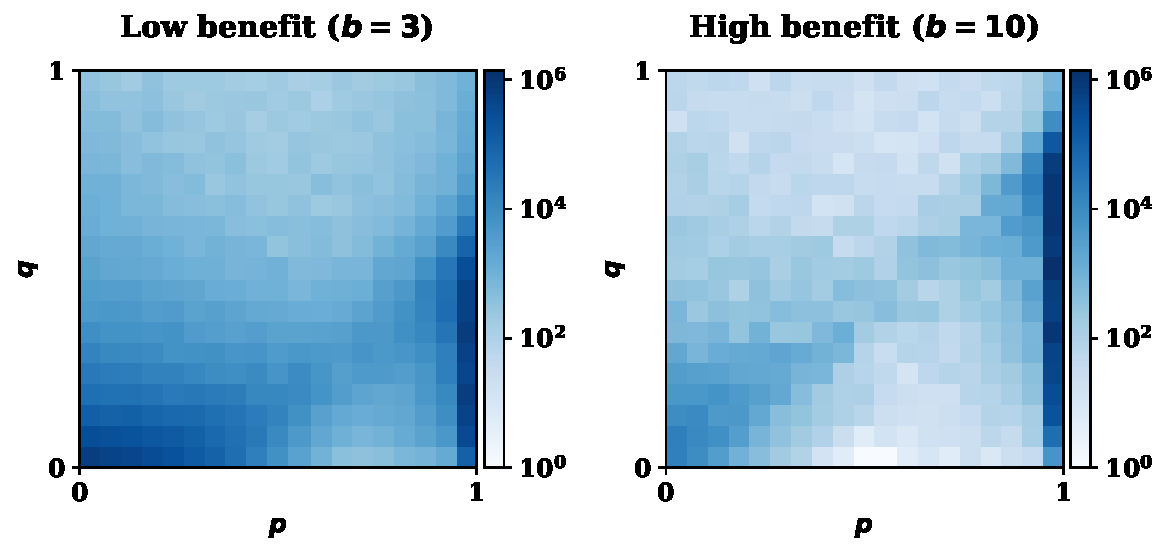
\includegraphics[width=.70\textwidth]{../static/expected_payoffs_donation_game.pdf}
    \caption{\textbf{Evolutionary dynamics under expected payoffs with
    low (left) and high (right) benefit.} We run the simulations for \(T =
    10^7\) time steps. For each time step, we have recorded the current resident
    population \((y, p, q)\). Since in the case of the expected payoffs the
    individuals interact for an infinite number of times \(\delta \rightarrow
    1\), we do not report the players' initial cooperation probability \(y\).
    The graphs show how often the resident population chooses each combination
    \((p, q)\) of conditional cooperation probabilities in the subsequent
    rounds. In both cases players update based on their expected payoffs (A) In
    the case where \(b=3\), the resident population either consists of defectors
    (with \(p \approx q \approx 0\)) or of conditional cooperators for which \(p
    \approx 1\) and \(q \leq 1 - \frac{1}{3}=0.7\). (B) In the case where
    \(b=10\), the resident population typically applies a strategy for which \(p
    \approx 1\) and \(q \leq 1 - \frac{1}{10}=0.9\). Parameters: \(N =100, c=1,
    \beta=1\).
    }\label{fig:expected_payoffs_results}
\end{figure}

\subsection{Updating Payoffs based on the one interaction - last round payoffs}

The first approach we introduced in this work is that of the one  interaction -
last round updating payoff. In this case an individual updates his strategy
based on the last payoff they received against the one other member of the
population. Initially, we define the payoff of a reactive strategy in the last
round at the stage game. This is given by
Proposition~\ref{proposition:last_round}.

\begin{Prop}\label{proposition:last_round} Consider a repeated game, with
    continuation probability $\delta$, between players with reactive strategies
    $s_1\!=\!(y_1, p_1, q_1$)  and $s_2\!=\!(y_2,p_2,q_2)$ respectively. Then
    the probability that the $s_1$ player receives the payoff $u\!\in\!
    \mathcal{U}$ in the very last round of the game is given by
    $v_{u}(s_1,s_2)$, as given by Equation~(\ref{Eq:LastRound}).

    \begin{equation} \label{Eq:LastRound}
      \setlength{\arraycolsep}{1pt}
      \begin{array}{rcl}
    
      v_{R}(s_1,s_2) &= &\displaystyle (1\!-\!\delta)\frac{y_1y_2}{1\!-\!\delta^2 r_1 r_2}+\delta \frac{\Big(q_1+r_1\big((1\!-\!\delta)y_2+\delta q_2\big)\Big) \Big(q_2+r_2\big((1\!-\!\delta)y_1+\delta q_1\big)\Big)}
      {\displaystyle(1\!-\!\delta r_1r_2)(1\!-\!\delta^2 r_1 r_2)} \times R,\\[1cm]
    
      v_{S}(s_1,s_2) &= &\displaystyle (1\!-\!\delta)\frac{y_1\bar{y}_2}{1\!-\!\delta^2 r_1 r_2}+\delta \frac{\Big(q_1+r_1\big((1\!-\!\delta)y_2+\delta q_2\big)\Big) \Big(\bar{q}_2+\bar{r}_2\big((1\!-\!\delta)y_1+\delta p_1\big)\Big)}
      {\displaystyle(1\!-\!\delta r_1r_2)(1\!-\!\delta^2 r_1 r_2)} \times S,\\[1cm]
    
      v_{T}(s_1,s_2) &= &\displaystyle (1\!-\!\delta)\frac{\bar{y}_1y_2}{1\!-\!\delta^2 r_1 r_2}+\delta \frac{\Big(\bar{q}_1+\bar{r}_1\big((1\!-\!\delta)y_2+\delta p_2\big)\Big) \Big(q_2+r_2\big((1\!-\!\delta)y_1+\delta q_1\big)\Big)}
      {\displaystyle(1\!-\!\delta r_1r_2)(1\!-\!\delta^2 r_1 r_2)} \times T,\\[1cm]
    
      v_{P}(s_1,s_2) &= &\displaystyle (1\!-\!\delta)\frac{\bar{y}_1\bar{y}_2}{1\!-\!\delta^2 r_1 r_2}+\delta \frac{\Big(\bar{q}_1+\bar{r}_1\big((1\!-\!\delta)y_2+\delta p_2\big)\Big) \Big(\bar{q}_2+\bar{r}_2\big((1\!-\!\delta)y_1+\delta p_1\big)\Big)}
      {\displaystyle(1\!-\!\delta r_1r_2)(1\!-\!\delta^2 r_1 r_2)} \times P.
      \end{array}
    \end{equation}

In these expressions, we have used the notation $r_i:=p_i\!-\!q_i$,
$\bar{y}_i\!=\!1\!-\!y_i$, $\bar{q}_i:=1\!-\!q_i$, and
$\bar{r}_i:=\bar{p}_i\!-\!\bar{q}_i=-r_i$ for $i\!\in\!\{1,2\}$.
\end{Prop}

Note that in the proposition we use the general notation of the prisoner's
dilemma, to denote that the results apply to \(2 \times 2\) any symmetric game.

\begin{proof}
Given a play between two reactive strategies with continuation probability
$\delta$. The outcome at turn \(t\) is given by,

\begin{equation}\label{eq:}
  (1 - \delta) \mathbf{v_0} \sum \delta^{t} M^{(t)},
\end{equation}

where $\mathbf{v_0}$ denotes the expected distribution of the four outcomes in
the very first round, and \(1- \delta\) the probability that the game ends. It
can be shown that,

\begin{align*}
  (1 - \delta) \mathbf{v_0} \sum \delta^{t} M^{(t)} & = (1 - \delta)(\mathbf{v_0} + \delta \mathbf{v_0} M + \delta^{2}\mathbf{v_0} M ^{2} + \dots )\\ 
   & = (1 - \delta)\mathbf{v_0} (1 + \delta M + \delta^{2}M ^{2} + \dots ) \text{ using standard formula for geometric series}\\ 
   & = (1 - \delta)\mathbf{v_0}(I_4 - \delta M)^{-1}
\end{align*}

where \((1 - \delta)\mathbf{v_0}(I_4 - \delta M)^{-1}\) is vector \(\in R^{4}\)
and it the probabilities for being in any of the outcomes \(CC, CD, DC, DD\) in
the last round. Combining this with the payoff vector \(u\) and some algebraic
manipulation we derive to the Equation~\ref{Eq:LastRound}.
\end{proof}

In the updating stage we select a mutant and resident to be either the role
model or the learner. Given that they can interact with only one other member of
the population, they can interact either with each other or either can interact
with another resident or with another mutant. Thus, in each updating stage there
are five possible combinations of pairs (Figure~\ref{fig:single_pairs}).

\begin{figure}[!htbp]
  \centering
  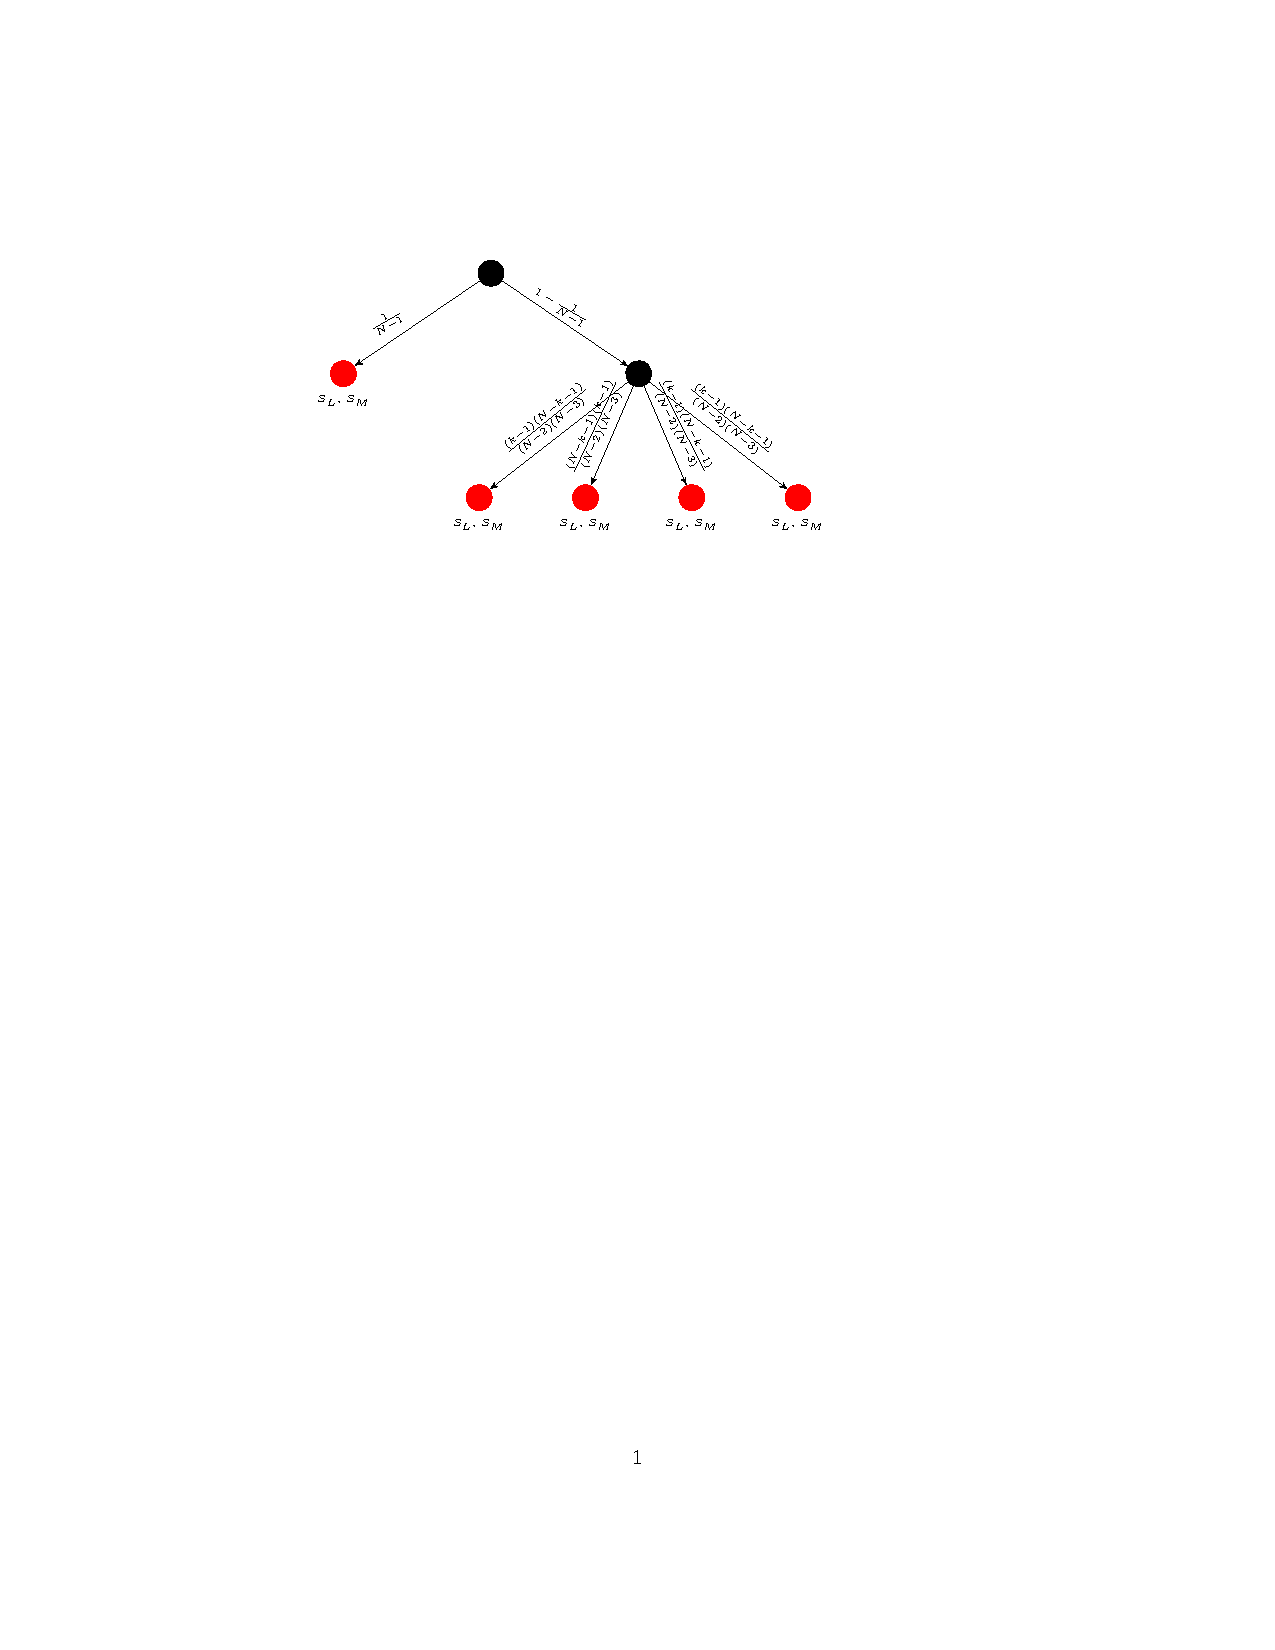
\includegraphics[width=.65\textwidth]{../static/last_rounds_matches.tex}
  \caption{\textbf{Possible pairings combination in the updating stage, given
  that individuals interact with only one other member in the population.} At
  each step of the evolutionary process we choose a role model and a learner to
  update the population. We consider the case where both the role model and the
  learner estimate their fitness after interacting with a single member of the
  population. There are five possible pairings at each step. They interact with
  other with a probability \(\frac{1}{N - 1}\), and thus they do not interact
  with other with a probability \(1 - \frac{1}{N - 1}\). In the latter case,
  each of them can interact with either a mutant or a resident. Both of them
  interact with a mutant with a probability $\frac{(k-1)(k-2)}{(N-2)(N-3)}$ and
  both interact with a resident with a probability
  $\frac{(N-k-1)(N-k-2)}{(N-2)(N-3)}$. The last two possible pairings are that
  either of them interacts with a resident whilst the other interacts with a
  mutant, and this happens with a probability
  $\frac{(N-k-1)(k-1)}{(N-2)(N-3)}$.}
  \label{fig:single_pairs}
\end{figure}

Given the last round payoff and possible pair combinations for a single
interaction, we define the probability that the respective last round payoffs of
two players \(s_1, s_2\) are given by $u_1$ and $u_2$ as,

\begin{equation}\label{eq:Chi}
\setlength{\arraycolsep}{1pt}
\begin{array}{llrl}
x(u_1,u_2)	 &=&\displaystyle \frac{1}{N\!-\!1}\cdot  &v_{u_1}(s_1,s_2)\cdot 1_{(u_1,u_2)\in \mathcal{U}^2_F}\\[0.5cm]
&+	
&\displaystyle \left(1\!-\!\frac{1}{N\!-\!1}\right)  
&\left[ \frac{k\!-\!1}{N\!-\!2}\frac{k\!-\!2}{N\!-\!3} v_{u_1}(s_1,s_2) v_{u_2}(s_2,s_2) + 
 \frac{k\!-\!1}{N\!-\!2}\frac{N\!-\!k\!-\!1}{N\!-\!3} v_{u_1}(s_1,s_2) v_{u_2}(s_2,s_1)\right.\\[0.5cm]
&&&\left. +\frac{N\!-\!k\!-\!1}{N\!-\!2}\frac{k\!-\!1}{N\!-\!3} v_{u_1}(s_1,s_1) v_{u_2}(s_2,s_2) + 
 \frac{N\!-\!k\!-\!1}{N\!-\!2}\frac{N\!-\!k\!-\!2}{N\!-\!3} v_{u_1}(s_1,s_1) v_{u_2}(s_2,s_1)\right].
\end{array}
\end{equation}

The first term on the right side corresponds to the case that the learner and
the role model happened to be matched during the game stage, which happens with
probability $\frac{1}{(N\!-\!1)}$. In that case, we note that only those payoff
pairs can occur that are feasible in a direct interaction,
$\splitatcommas{(u_1,u_2)\in \mathcal{U}^2_F:=\big\{ (b-c, b-c), (-c, b), (b, -c), (0, 0)
\big\}}$, as represented by the respective indicator function. Otherwise, if the
learner and the role model did not interact directly, we need to distinguish
four different cases, depending on whether the learner was matched with a
resident or a mutant, and depending on whether the role model was matched with a
resident or a mutant.

Given that $N\!-\!k$ players use the resident strategy
$s_{R}\!=\!(y_{R},p_{R},q_{R})$ and that the remaining $k$ players use the
mutant strategy $s_{M}\!=\!(y_{M},p_{M},q_{M})$, the probability that the number
of mutants increases by one in one step of the evolutionary process can be
written as

\begin{align}
\lambda^+_k=\frac{N\!-\!k}{N}\cdot \frac{k}{N}\cdot \sum_{u_{R},u_{M}\in\mathcal{U}} x(u_{R},u_{M})\cdot \rho(u_{R},u_{M}), \\
\lambda^-_k=\frac{N\!-\!k}{N}\cdot \frac{k}{N}\cdot \sum_{u_{R},u_{M}\in\mathcal{U}} x(u_{R},u_{M})\cdot \rho(u_{M},u_{R}).
\end{align}

In this expression, $\frac{(N\!-\!k)}{N}$ is the probability that the randomly
chosen learner is a resident, and $\frac{k}{N}$ is the probability that the role
model is a mutant. The sum corresponds to the total probability that the learner
adopts the role model's strategy over all possible payoffs $u_R$ and $u_M$ that
the two player may have received in their respective last rounds. We use
$x(u_R,u_M)$ to denote the probability that the randomly chosen resident
obtained a payoff of $u_R$ in the last round of his respective game, and that
the mutant obtained a payoff of $u_M$.


\subsubsection{Invasion analysis of ALLD into (GTFT)}

Similarly to the previous section, we calculate how easily a single ALLD mutant
can invade into a resident population with strategy GTFT.

When two GTFT players interact in the game, their respective probabilities for
each of the four outcomes in the last round simplify to,

\begin{align*}
    v_R(GTFT,GTFT) = 1, & \quad v_T(GTFT,GTFT) = 0, \\
    v_S(GTFT,GTFT) = 0, & \quad v_P(GTFT,GTFT) = 0.
\end{align*}

On the other hand, if an ALLD player interacts with a GTFT player, the
respective probabilities according to Eq.~\ref{Eq:LastRound} become

\begin{align*}
    v_R(ALLD,GTFT) & = 0, &  v_S(ALLD,GTFT) & = 0, \\
    v_T (ALLD, GT F T ) & = 1 - \delta + \delta q, &  v_P (ALLD, GTFT) & = \delta(1 - q).
\end{align*}

As a consequence, we obtain the following probabilities \(x(u_1, u_2)\) that the
payoff of a randomly chosen GTFT player is \(u_1\) and that the payoff of the
ALLD player is \(u_2\),

\begin{align*}
  x(R, T) = & \frac{N - 2}{N - 1} \cdot (1 - \delta + \delta q)\\
  x(R, R) = & \frac{N - 2}{N - 1} \cdot \delta (1 - q) \\
  x(S, T) = & \frac{1}{N - 1} \cdot (1 - \delta + \delta q) \\
  x(P, P) = & \frac{1}{N - 1} \cdot \delta (1 - q)
\end{align*}

As a consequence, we can calculate the ratio of transition probabilities as

\begin{equation*}
  \resizebox{.9\textwidth}{!} 
  {$
    \frac{\lambda^{+}}{\lambda^{-}} = \frac{\frac{N - 2}{N - 1} \cdot \left(\frac{\delta(1-q)}{e^{-\beta(c - b)} + 1} + \frac{-\delta +\delta  q + 1}{e^{-\beta c} + 1}\right) + \frac{1}{N - 1} \cdot \left(\frac{-\delta +\delta  q+1}{e^{\beta  (-(b+c))}+1}\right)}
    {\frac{N - 2}{N - 1} \cdot \left(\frac{\delta (1-q)}{e^{-\beta (b-c)}+1} + \frac{-\delta +\delta  q + 1}{e^{\beta  c}+1}\right)+ \frac{1}{N-1} \cdot \left(\frac{-\delta +\delta  q+1}{e^{-\beta  ((-b-c))}+1}\right)}
  $}
\end{equation*}

In particular, in the limit of strong selection \(\beta \rightarrow \infty\) and
large populations \(N \rightarrow \infty \), we obtain

\begin{equation*}
    \frac{\lambda^{+}}{\lambda^{-}} = \frac{1 - \delta + \delta q}{\delta(1 - q)}
\end{equation*}

This ratio is smaller than 1 (such that ALLD is disfavored to invade) if \(q <
1- 1/(2 \delta)\). For infinitely repeated games, \(\delta \rightarrow 1\), this
condition becomes \(q < 1/2\) (for \(q = 1/2\), the payoff of the ALLD player is
\(T > R\) for half of the time, and it is \(P < R\) for the other half. The
probability that the number of mutants increase by one equals the probability
that the mutant goes extinct).

\subsubsection{Simulation results}

In a similar fashion to Section~\ref{section:simulation_results_exprected}, we
simulate the evolutionary process given that individuals now use the last
interaction-last round payoffs to update their strategies.
Figure~\ref{fig:one_interaction_last_round_payoffs_results} shows simulation
results. Though, a higher benefit results in a more cooperative population, in
the case of these updating payoff, only to a slightly more cooperative. As shown
in Figure~\ref{fig:one_interaction_last_round_payoffs_results} the evolving
populations are more similar, both consisting of defectors and conditional
cooperators. Compared to the expected payoffs, the conditional cooperators are
also less cooperative \(p \approx 1\) and \(q \leq \frac{1}{2}\). The increased
benefit pushes the population closer to the boundary of \(q \leq \frac{1}{2}\)
but that is the maximum.

\begin{figure}[!htbp]
  \centering 
  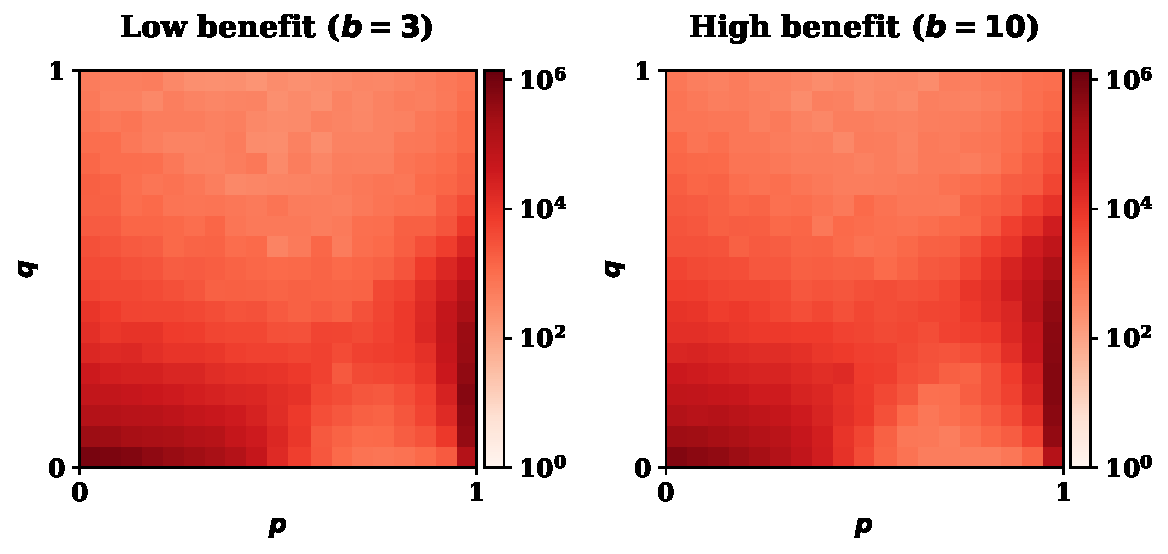
\includegraphics[width=.70\textwidth]{../static/one_interaction_last_round_payoffs_results}
  \caption{\textbf{Evolutionary dynamics under one interaction last round
  payoffs with low (left) and high (right) benefit.} In the cases of low and
  high benefit case the resident population either consists of defectors (with
  \(p \approx q \approx 0\)) or of conditional cooperators for which \(p \approx
  1\) and \(q \leq \frac{1}{2}\). Parameters: \(N =100, c=1, \beta=1\).
  }\label{fig:one_interaction_last_round_payoffs_results}
\end{figure}

\subsection{Updating Payoffs based on \(n\) interactions - last \(m\) round payoffs}

So far we have presented the two extreme cases; the case where an individual
updates based one interaction and one round, and the case  where an individual
updates based on all interactions and all rounds. In this work we also
explore the intermediate cases (Figure~\ref{fig:cases_updating_payoffs}). Namely the cases:

\begin{itemize}
  \item last round \(n=1\) with two other players \(m=2\)
  \item last two rounds \(n=2\) with one other player  \(m=1\)
  \item last two rounds \(n=2\) with two other players \(m=2\)
\end{itemize}

\begin{figure}[!htbp]
  \centering
  \includestandalone[width=.5\textwidth]{cases}
  \caption{\textbf{Updating payoffs used in this work.} \(n\) is the
  number of turns and \(m\) th number of individuals. The expected payoffs
  are the one commonly used in the literature. We have introduced a method
  for the rest.}\label{fig:cases_updating_payoffs}
\end{figure}

We define the payoffs on the two last round, and in the updating phase the
probability that.

We extend our framework to consider the case where players update their
strategies based on the outcome of \textbf{the last two turns and based on their
interaction with two other members of the population}. At the stage game we
define the payoff of a reactive strategy in the last two rounds,
Proposition~\ref{proposition:last_two_rounds}.

\begin{Prop}\label{proposition:last_two_rounds} Consider a repeated game, with
  continuation probability $\delta$, between players with reactive strategies
  $s_1\!=\!(y_1, p_1, q_1$)  and $s_2\!=\!(y_2,p_2,q_2)$ respectively. Let
  $\mathcal{\tilde{U}} = \splitatcommas{\{RR, RS, RT, RP, SR, SS, ST, SP, TR,
  TS, TT, TP, PR, PS, PT, PP\}}$ denote the set of feasible payoffs in the last
  two rounds, and let \(\tilde{\mathbf{u}}\) be the corresponding payoff vector.
  Then the probability that the $s_1$ player receives the payoff $u\!\in\!
  \mathcal{\tilde{U}}$ in the very last two rounds of the game is given by,

  \begin{equation}
  \langle\mathbf{\tilde{v}}(s_1,s_2),\mathbf{\tilde{u}}\rangle, \text{ where } \mathbf{\tilde{v}} \in R^{16} \text{ is given by },
  \end{equation}
  \begin{equation}
    \mathbf{\tilde{v}}(s_1,s_2) = (1 - \delta) m_{a_1, a_2} \delta^2 \left[\mathbf{v_0}(I_4 - \delta M)^{-1}\right]_{a_1, a_2}, \quad  m_{a_1, a_2} \in M \ \forall \ a_1, a_2 \in \{1, 2, 3, 4\}.
  \end{equation}
\end{Prop}

In the updating stage we select a mutant and resident to be either the role
model or the learner. Given that they can interact with two other members of the
population there are a total of twenty four possible combinations of pairs
(Figure~\ref{fig:pissible_two_pairs}).

\begin{figure}[!htbp]
  \centering
  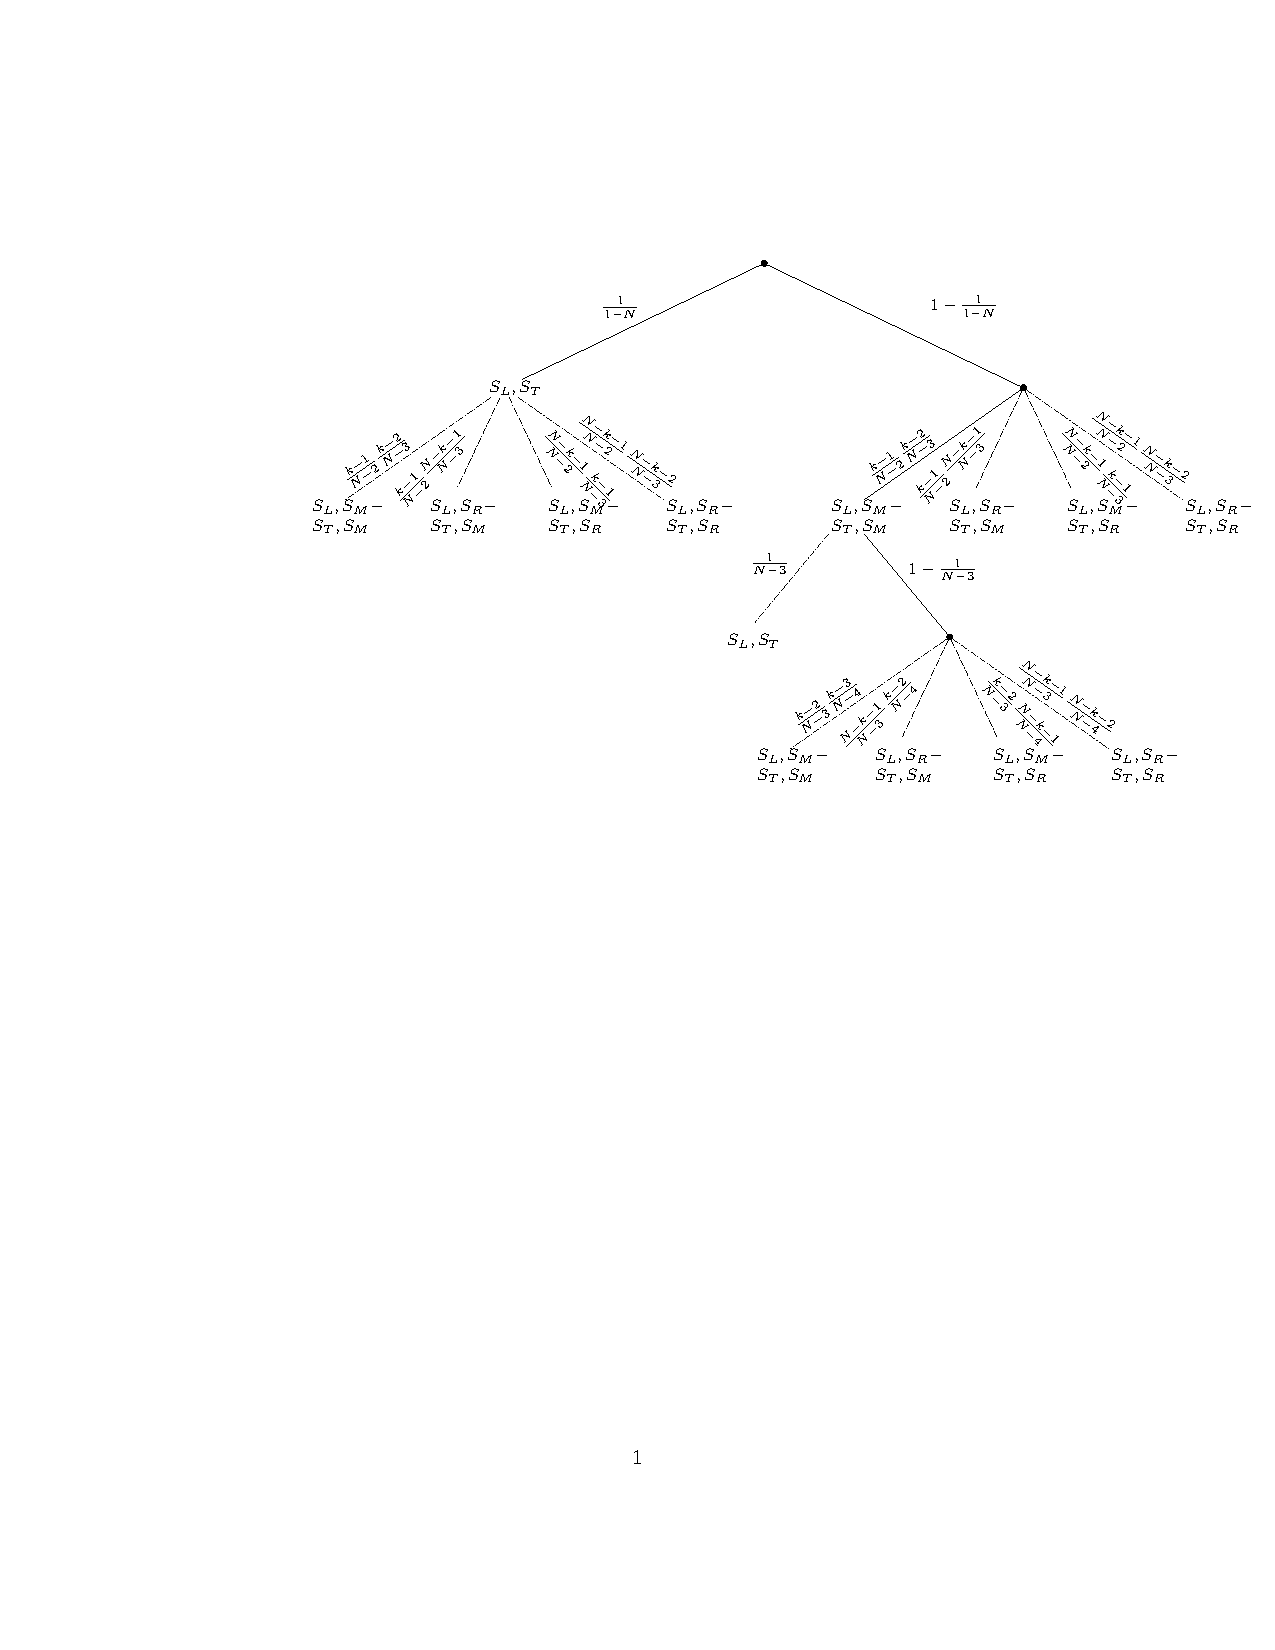
\includegraphics[width=.65\textwidth]{../static/tree.tex}
  \caption{\textbf{Possible pairings combination in the updating stage, given
  that individuals interact with two other members in the population.}}
  \label{fig:pissible_two_pairs}
\end{figure}

For the above cases we use combinations of Eq. 1 2 and 3.






\end{document}